% DO NOT COMPILE THIS FILE DIRECTLY!
% This is included by the other .tex files.

\begin{frame}[t,plain]
\titlepage
\end{frame}

\begin{frame}[t]{Resource Allocation}
    \begin{itemize}
        \item<2-> Allocation of scarce resources to \textbf{customers} under some constraints
        \item<3-> Application:
        \item<4->[ ]
        \begin{figure}
            \begin{subfigure}[b]{0.45\textwidth}  
                \centering
                
\includegraphics[width=2cm]{auction.eps}
                \caption*{Auctions}
                \label{fig:my_label}
            \end{subfigure}
            \begin{subfigure}[b]{0.45\textwidth}    
                \centering
                
\includegraphics[width=2cm]{pie-chart.eps}
                \caption*{Cake Cutting}
                \label{fig:my_label}
            \end{subfigure}
            \begin{subfigure}[b]{0.45\textwidth}     
                \centering
                
\includegraphics[width=2cm]{cpu.eps}
                \caption*{Job Scheduling}
                \label{fig:my_label}
            \end{subfigure}
            \begin{subfigure}[b]{0.45\textwidth}      
                \centering
                
\includegraphics[width=2cm]{delivery-truck.eps}
                \caption*{Delivery}
                \label{fig:my_label}
            \end{subfigure}
        \end{figure}
    \end{itemize}    
\end{frame}

\begin{frame}[t]{Resource Allocation Types}
    \begin{itemize}
        \item<2-> Divisible Resource Allocation
            \begin{itemize}
                \item<3-> Example: cake cutting problem
            	\item<4-> The question: \emph{fair division} of divisible resources
            	\item<5-> Mostly studied in  economics, game theory, and sociology
            \end{itemize}
        \item<6-> Indivisible Resource Allocation (\alert{IRA})
            \begin{itemize}
                \item<7-> Example: Auctions, Scheduling, Vehicle Routing
                \item<8-> Combinatorial nature of the allocation
                \item<9-> Mostly studied in operation research, combinatorial optimization, and computer science
            \end{itemize}  
    \end{itemize}
\end{frame}

\begin{frame}{In This Presentation}
  \tableofcontents
\end{frame}

%__________________________________________________________________________________
\section{Skill Vehicle Routing Problem}
\frame{\insertsection}

\begin{frame}[t]{Introduction (1)}
    \begin{minipage}[t]{0.48\textwidth}
        \begin{itemize}
            \item<1-> Set of \textbf{customers} $S$
            \item<2-> Skill requirement $q_j$,  $\forall j \in S$
            \item<3-> Fleet of vehicles (\textbf{drivers}) $D$
            \item<4-> Set of skills $K_i$ $\forall i \in D$
            \item<5-> Metric graph $G = (S, \, E)$
            \item<6-> Special node \emph{depot}, $r \in S$
            \item<7-> Cost function $c:E \rightarrow \bR^+$ for every pair of nodes
        \end{itemize}
    \end{minipage}
    \begin{minipage}[t]{0.48\textwidth}
        \begin{figure}
            \centering
            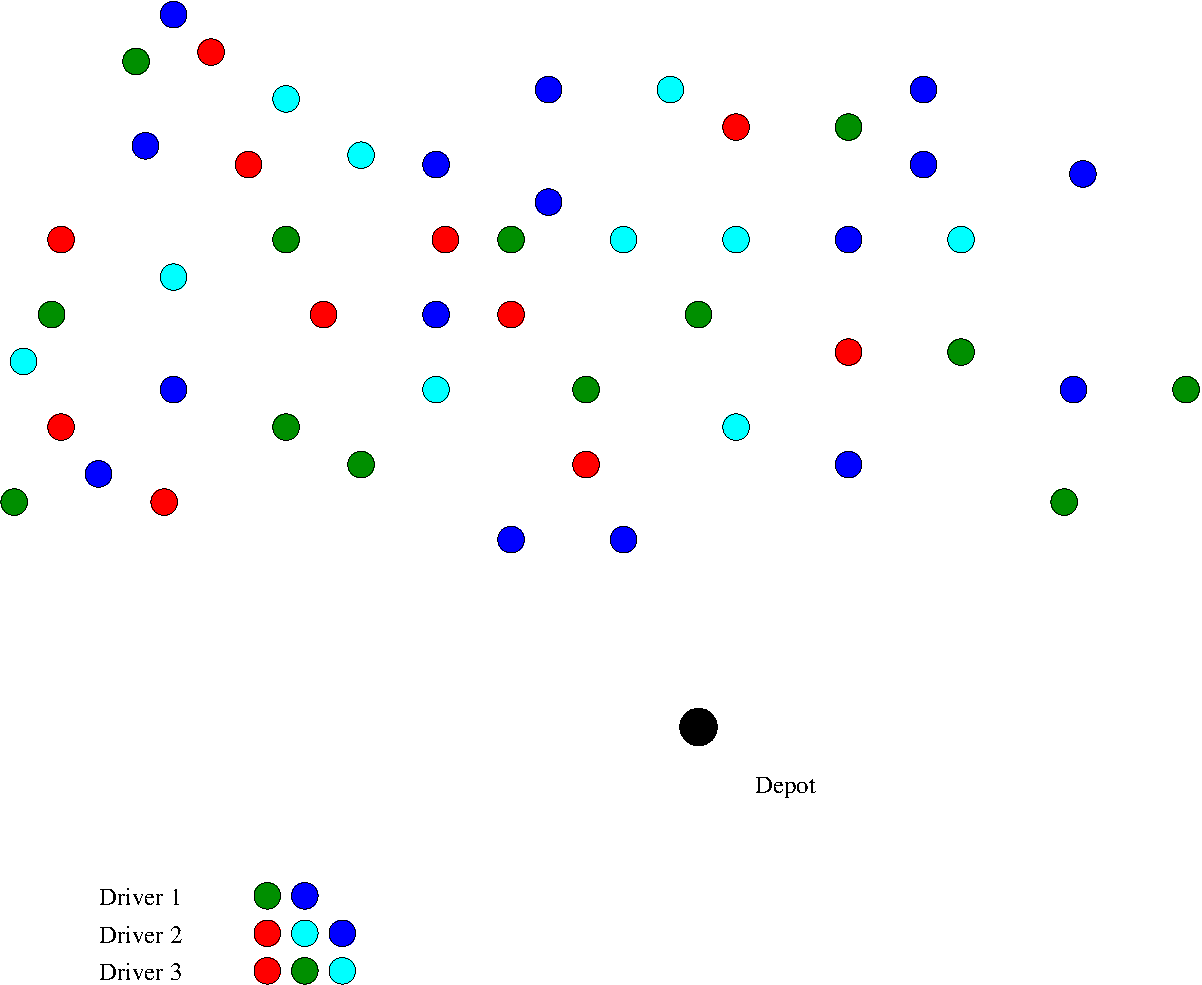
\includegraphics[width=5cm]{VRPSS01.pdf}
            \caption{SVRP}
            \label{fig:VRPSS01}
        \end{figure}            
    \end{minipage}
\end{frame}

\begin{frame}[t]{Introduction (1)}
    \begin{minipage}[t]{0.48\textwidth}
        \begin{itemize}
            \item Set of \textbf{customers} $S$
            \item Skill requirement $q_j$,  $\forall j \in S$
            \item Fleet of vehicles (\textbf{drivers}) $D$
            \item Set of skills $K_i$ $\forall i \in D$
            \item Metric graph $G = (S, \, E)$
            \item Special node \emph{depot}, $r \in S$
            \item Cost function $c:E \rightarrow \bR^+$ for every pair of nodes
        \end{itemize}
    \end{minipage}
    \begin{minipage}[t]{0.48\textwidth}
        \begin{figure}
            \centering
            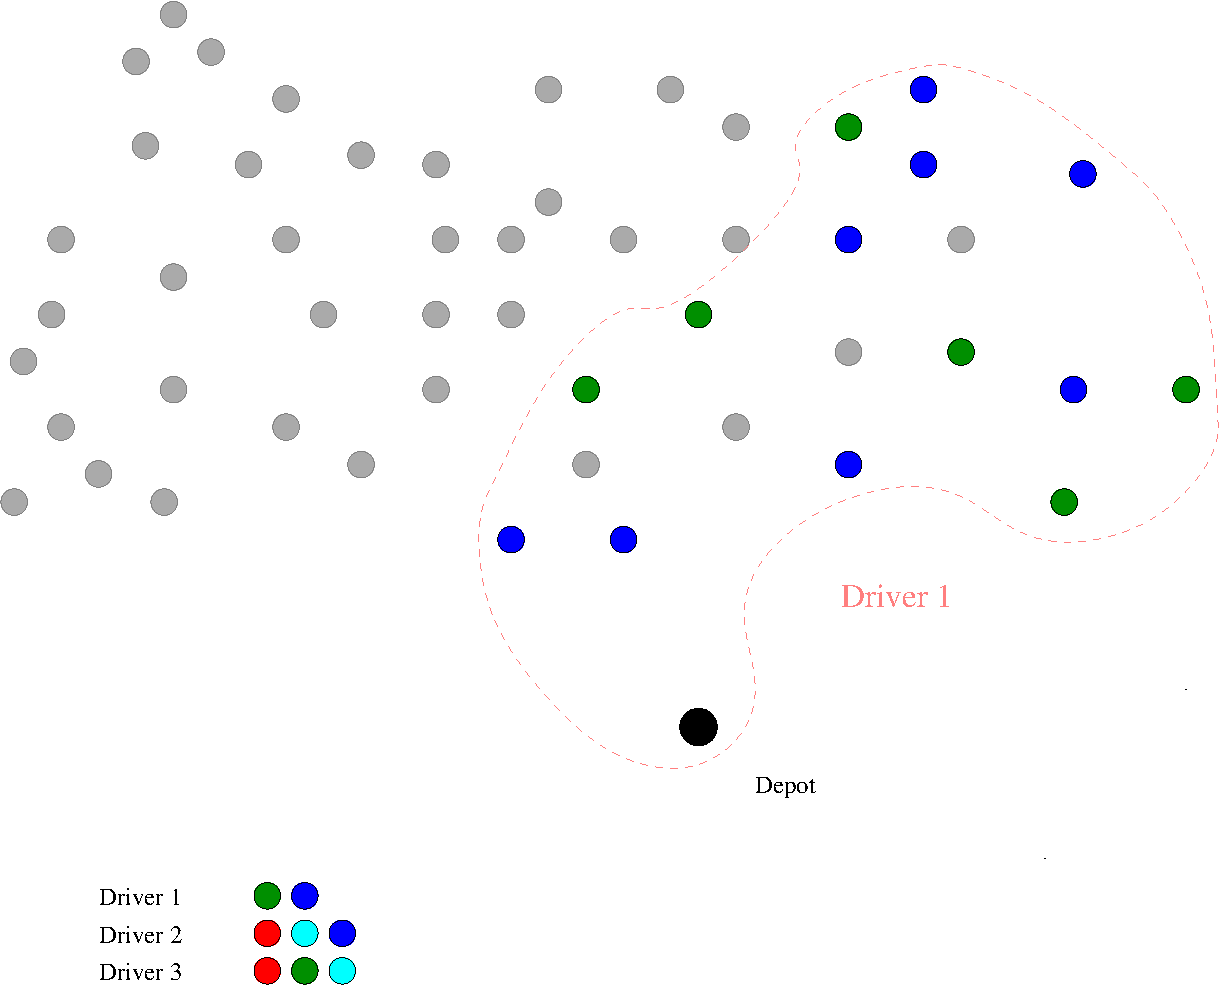
\includegraphics[width=5cm]{VRPSS02.pdf}
            \caption{SVRP}
            \label{fig:VRPSS02}
        \end{figure}            
    \end{minipage}    
\end{frame}

\begin{frame}[t]{Introduction (1)}
    \begin{minipage}[t]{0.48\textwidth}
        \begin{itemize}
            \item Set of \textbf{customers} $S$
            \item Skill requirement $q_j$,  $\forall j \in S$
            \item Fleet of vehicles (\textbf{drivers}) $D$
            \item Set of skills $K_i$ $\forall i \in D$
            \item Metric graph $G = (S, \, E)$
            \item Special node \emph{depot}, $r \in S$
            \item Cost function $c:E \rightarrow \bR^+$ for every pair of nodes
        \end{itemize}
    \end{minipage}
    \begin{minipage}[t]{0.48\textwidth}
        \begin{figure}
            \centering
            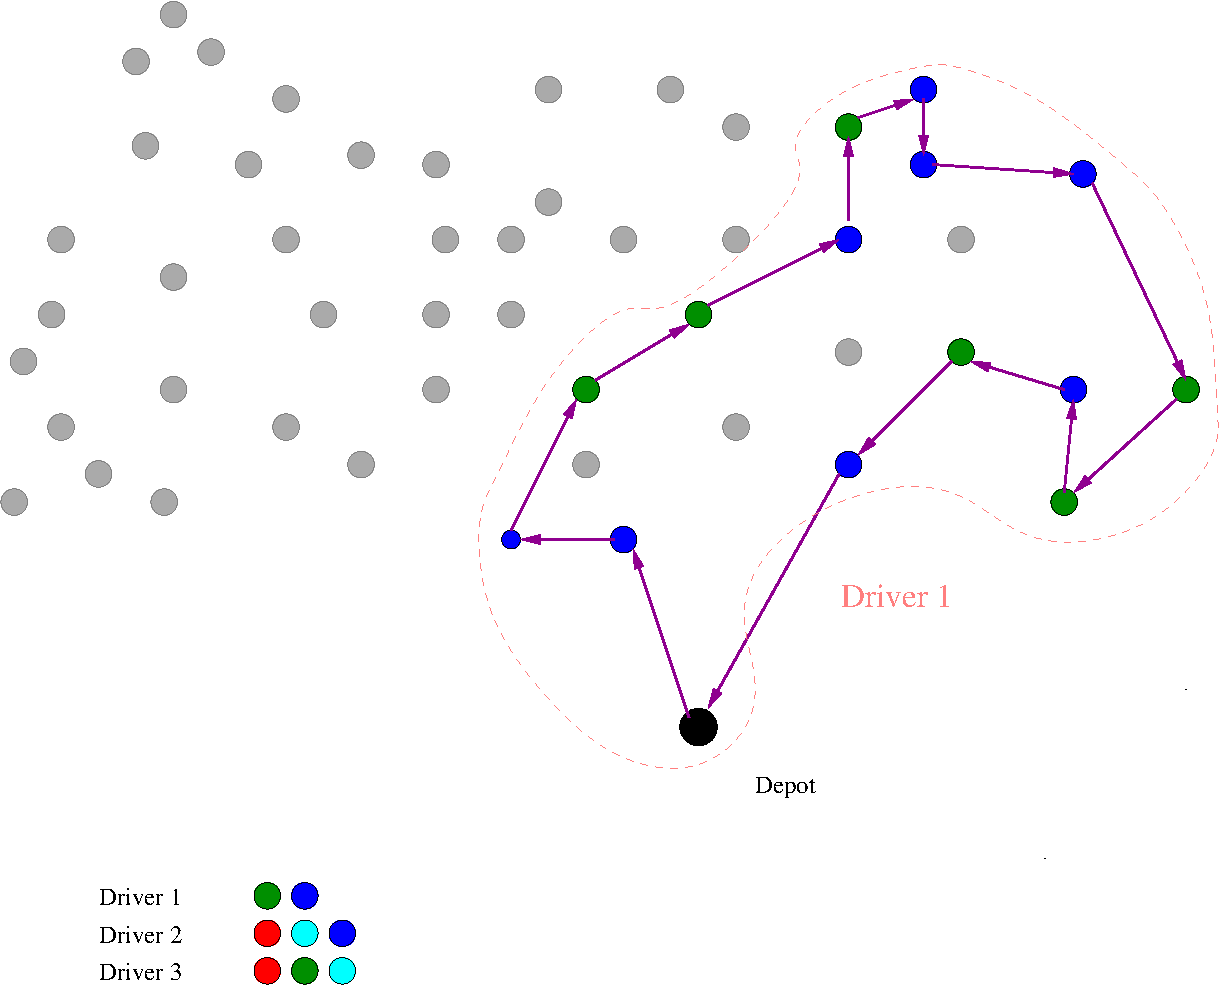
\includegraphics[width=5cm]{VRPSS03.pdf}
            \caption{SVRP}
            \label{fig:VRPSS02}
        \end{figure}            
    \end{minipage}    
\end{frame}

\begin{frame}{Introduction (2)}
\begin{itemize}
    \item<1-> Goal: to find \textbf{tours} (routes that start and end at $r$) and assign them to drivers such that:
    \begin{itemize}
        \item<2-> The union of all the tours cover $S$
        \item<3-> The drivers can served the customers assigned to them
        \item<4-> The total travel distance is minimized
    \end{itemize}
    \item<5-> SVRP has immediate applications in logistics and transportation
        \begin{itemize}
            \item<6-> Transport costs account for 10\% of the total cost of a product
            \item<7-> Manual optimization of the transport cost becomes infeasible as the scale grows
        \end{itemize}
    \item<7-> We seek to solve SVRP \textbf{computationally}
\end{itemize}
\end{frame}


\begin{frame}[t]{Solution Methods}
    \begin{itemize}
        \item<1-> Metaheuristics:
            \begin{itemize}
                \item<2-> Tabu search
                \item<3-> Simulated annealing
                \item<4-> \ldots
            \end{itemize}
        \item<5-> Linear Programming:
            \begin{itemize}
                \item<6-> Goal: obtain minimum-cost solutions or lower and upper bounds
                \item<7-> an LP-relaxation used in a branch-and-bound algorithm
                \item<8-> Integrality gap plays an important role
                \item<9-> Question: a formulation with small gap?
                \item<10-> Answer: \textbf{Configuration LP}
            \end{itemize}
    \end{itemize}
\end{frame}

\begin{frame}[t]{Configuration LP (1)}
    \begin{itemize}
        \item<1-> First used in the context of Bin Packing problems
        \item<2-> Define $\cT(i)$: set of tours that $i$ can serve        
        \item<3-> For every driver $i \in D$ and every tour $T \in \cT(i)$:
        \[
            z_{i, T} =
                \begin{cases}
                    1 & \text{if driver $i$ visits the vertices in the tour $T$} \\
                    0 & \text{otherwise}
                \end{cases}
        \]
    \end{itemize}
\end{frame}
\begin{frame}[t]{Configuration LP (2)}
    \label{CLP2}
    \begin{itemize}
        \item<1->[ ] \begin{align}
            \text {min } \label{cg_obj}	 \sum_{ i, 	T \in \cT(i) } z_{i, T} & \cdot C(T) &    &  \\
            \text{subject to }             & & \nonumber  \\
            \label{const:cg1}       \sum_{ T \in \cT(i) } z_{ i, T } & = 1  &   \forall i \in D \\
            \label{const:cg2}       \sum_{ i, T \in \cT(i): T \ni j } & z_{ i, T } & \geq 1   &   \forall j \in S \\
            \label{consT:cg3}       z_{ i, T } & \in \{0,\, 1\}    & \forall \, i \in D, \, \forall \, T \in \cT(i) 
        \end{align}        
        \hyperlink{our_method_bp}{\beamergotobutton{Branch-and-Price}}
    \end{itemize}
\end{frame}

\begin{frame}[t]{Configuration LP (3)}
    \begin{itemize}
        \item<1-> Advantage:
            \begin{itemize}
                \item<2-> Small integrality gap
            \end{itemize}
        \item<3-> Disadvantage: 
            \begin{itemize}
                \item<4-> Exponential number of variables
            \end{itemize}
        \item<5-> Common technique for dealing with LP formulations with a large number of constraints: \textbf{Delayed Column Generation}
            \begin{itemize}
                \item<6-> Do not introduce all the variables at once
                \item<7-> Solve LP relaxation on a subset of variables (columns)
                \item<8-> Detect and introduce columns that can improve the solution: \textbf{reduced-cost columns}
                \item<9-> Used extensively for Vehicle Routing Problems with Time Windows
            \end{itemize}
    \end{itemize}
\end{frame}

\begin{frame}[t]{Our Contributions}
    \label{our_method_bp}
    \begin{itemize}
        \item<1-> A \alert{Branch-and-Price} algorithm: 
        \item<2-> Use column generation in a branch-and-bound framework
        \item<3-> Detect the reduced-cost columns (\textbf{Pricing} subproblem)
            \begin{itemize}
                \item<4-> Exact solutions: \alert{Prize-Collecting TSP}
                \item<5-> Heuristic: a \alert{local search} algorithm 
            \end{itemize}
        \item<6-> Use both the exact and heuristic solution to improve upper and lower bounds \hyperlink{CLP2}{\beamergotobutton{Config. LP}}        
        \item<7-> Future projects:
            \begin{itemize}
                \item<8-> Benchmarking heuristics and metaheuristics
                \item<9-> Improving the branch-and-price with heuristics
            \end{itemize}
    \end{itemize}
\end{frame}

%__________________________________________________________________________________
\section{Prize Collecting TSP}
\frame{\insertsection}

\begin{frame}[t]{Introduction}

\begin{itemize}
\item<1-> A variant of the Traveling Salesman Problem (TSP)
\item<2-> Metric graph $G = (S, \, E)$ (on a Euclidean plane) 
\item<3-> A special node depot, $r \in S$
\item<4-> A cost function $c:E \rightarrow \bR^+$ for every pair of nodes
\item<5-> A prize function $\beta:S \rightarrow \bR^+$ for every node
\item<6-> Objective: Find a tour covering the depot and a \emph{subset} of nodes, maximizing the sum of prizes minus the sum of costs

\end{itemize}
\end{frame}

\begin{frame}[t]{Introduction (2)}

\begin{itemize}
\item An instance of the Prize Collecting TSP:
\begin{figure}
	\centering
	\begin{tikzpicture}
        
        \draw (0, 0) node[circle, inner sep=1pt, fill=black, label={below:{$depot$}}] (D) {}; 
        \draw (1, 1) node[circle, inner sep=1pt, fill=black] (A) {}; 
        \draw (3, 2) node[circle, inner sep=1pt, fill=black] (B) {}; 
        \draw (-3, 3) node[circle, inner sep=1pt, fill=black] (C) {}; 
        \draw (-1, 4) node[circle, inner sep=1pt, fill=black] (E) {}; 
        \draw (0, 3) node[circle, inner sep=1pt, fill=black] (F) {}; 
        \draw (2, 3) node[circle, inner sep=1pt, fill=black] (G) {}; 
         \draw (-3, 1) node[circle, inner sep=1pt, fill=black, label={below:{$v$}}] (v) {}; 
        \draw (-2, 2) node[circle, inner sep=1pt, fill=black, label={below:{$u$}}] (u) {};         
        \node at (-2.5, 1.5) (m) {};
        \node at (-4, 1.5) (n) {$c_{uv}$};
        
        \draw [->, color = red] (m) to [bend right = 45] (n);
        \draw [fill = blue, dashed, thick] (u) to (v);

    	\node[above = 0.2cm] at (-2, 2) {$\beta_u$};
	\end{tikzpicture}
    \caption{Prize Collecting TSP}
    \label{fig:intersect_intervals}
\end{figure}
\end{itemize}
\end{frame}

\begin{frame}[t]{Introduction (3)}

\begin{itemize}
\item Solution value $ = (6 + 2 + 7 + 10 + 4) - (3.2  + 1.4 + 2.2 + 3.2 + 2.2 + 1.4) = $ \alert{15.4}
\begin{figure}
	\centering
	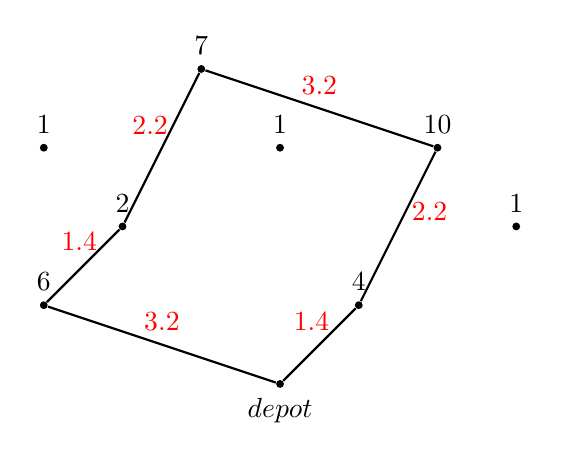
\begin{tikzpicture}
        
        \draw (0, 0) node[circle, inner sep=1pt, fill=black, label={below:{$depot$}}] (D) {}; 
        \draw (1, 1) node[circle, inner sep=1pt, fill=black, label = {above:{4}}] (A) {}; 
        \draw (3, 2) node[circle, inner sep=1pt, fill=black, label = {above:{1}}] (B) {}; 
        \draw (-3, 3) node[circle, inner sep=1pt, fill=black, label = {above:{1}}] (C) {}; 
        \draw (-1, 4) node[circle, inner sep=1pt, fill=black, label = {above:{7}}] (E) {}; 
        \draw (0, 3) node[circle, inner sep=1pt, fill=black, label = {above:{1}}] (F) {}; 
        \draw (2, 3) node[circle, inner sep=1pt, fill=black, label = {above:{10}}] (G) {}; 
         \draw (-3, 1) node[circle, inner sep=1pt, fill=black, label = {above:{$6$}}] (v) {}; 
        \draw (-2, 2) node[circle, inner sep=1pt, fill=black, label = {above:{$2$}}] (u) {};                 
        \draw [fill = blue, thick] (D) to (v) to (u) to (E) to (G) to (A) to (D);
        \node [above = 0.05cm, color = red] at (-1.5, 0.5) {3.2};
        \node [above = 0.07cm, color = red] at (-2.55, 1.5) {1.4};
        \node [above = 0.05cm, color = red] at (-1.65, 3) {2.2};
        \node [above = 0.05cm, color = red] at (0.5, 3.5) {3.2};
        \node [above = 0.05cm, color = red] at (1.9, 1.9) {2.2};
        \node [above = 0.05cm, color = red] at (0.4, 0.5) {1.4};
        
	\end{tikzpicture}
    \caption{A feasible solution to PCTSP}
    \label{fig:intersect_intervals}
\end{figure}
\end{itemize}
\end{frame}

\begin{frame}[t]{Solution Methods}
    \begin{itemize}
        \item<1-> PCTSP may arise as subproblem in a column generation technique for many vehicle routing problems
        \item<2-> SVRP is one example
        \item<3-> We seek:
            \begin{itemize}
                \item<4-> Fast heuristics that provide near-optimal solutions
                    \begin{itemize}
                        \item<5-> These solutions can be used as reduced-cost columns for SVRP
                        \item<6-> Normally based on local search
                    \end{itemize}
                \item<7-> Exact solutions that provide bounds for SVRP
                    \begin{itemize}
                        \item<8-> Based on LP formulations with small integrality gap
                        \item<9-> Used in a branch-and-bound framework
                    \end{itemize}
                    
            \end{itemize}
    \end{itemize}
\end{frame}


\begin{frame}[t]{Related Work}
\begin{itemize}
    \item<1-> Metaheuristics:
        \begin{itemize}
            \item<2-> A local search algorithm is due to Chaves and Lorena
        \end{itemize}
        \item<3-> Linear Programming:
        \begin{itemize}
            \item<4-> Some formulations with exponential number of constraints exhibit low integrality gaps for TSP-like problems
            \item<5-> Normally a mix of cutting plane method and branch-and-bound is used: \textbf{Branch-and-Cut}
            \item<6-> Gendreau et al., Fischetti et al., and Laporte et al. provide Branch-and-Cut algorithms for variants of the problem
        \end{itemize}
\end{itemize}
\end{frame}

\begin{frame}[t]{ILP Formulation (1)}
    \begin{itemize}
        \item<1-> Two sets of decision variables:
        \item<2-> For every vertex $i \in S$:
        \[
            y_j =
                \begin{cases}
                    1 & \text{if vertex $j$ is selected in the optimal tour} \\
                    0 & \text{otherwise}
                \end{cases}
        \]       
        \item<3-> For every edge $e \in E$:
        \[
            x_e =
                \begin{cases}
                    1 & \text{if edge $e$ is selected in the optimal tour} \\
                    0 & \text{otherwise}
                \end{cases}
        \]        
    \end{itemize}
\end{frame}

\begin{frame}[t]{ILP Formulation (2)}
    \begin{align} 
        \text {max } \label{pctsp_obj}     & \sum_{j\in S} \beta_j y_j  -     \sum_{e\in E} c_e x_e &
        \\
        \text{subject to } \nonumber    &  & \\
        \label{const:pctsp1}               & \sum_{e \in \delta(i)} x_e = 2 y_{i}  & \forall i \in S \\
        \label{const:pctsp2}               & \sum_{e \in E(V) } x_e \leq \sum_{i \in V \backslash\{ k \}} y_{i} & \forall k \in V, V\subseteq S' \\
        \label{const:pctsp3}               & y_r = 1 \\
        \label{const:pctsp4}               & x_e \in \{0, \, 1\}, \, y_j \in \{0, \, 1\}  
    \end{align}
\end{frame}

\begin{frame}[t]{ILP Formulation (3)}
    \begin{itemize}
        \item<1-> \constref{pctsp2} are referred to as the \textbf{Generalized Subtour Elimination Constraints} (GSECs) 
        \item<2-> Problem: there are exponentially many GSECs
        \item<3-> Solution: do not introduce them all at once (cutting plane method)
            \begin{itemize}
                \item<4-> Start with an initial set of constraints and solve the LP relaxation
                \item<5-> Identify violated constrains (if any) and add them to the model
                \item<6-> Iterate until completion
            \end{itemize}    
    \end{itemize}
\end{frame}

\begin{frame}[t]{Our Contributions}
\end{frame}

%__________________________________________________________________________________
\section{Ordered Instances of the Scheduling Problem}
\frame{\insertsection}



\begin{frame}[t]{What is this?}
\begin{itemize}
\item Beamer is a \LaTeX{} class that allows you to create presentations
\item The project home page is http://latex-beamer.sourceforge.net/
\item Beamer contains several themes, but they are a bit ugly
  \begin{itemize}
  \item But with a lot of useful features, such as navigation bars, outlines,
        etc.
  \end{itemize}
\item Torino is a pretty theme
  \begin{itemize}
  \item With a lot of useless -- but pretty -- features
  \item But without some useful features
  \item Well suited for short talks, for longer talks you should use themes
        with navigation bars
  \end{itemize}
\item Why the name?
  \begin{itemize}
  \item Other themes are named after locations of Universities or conferences
  \item Torino (Turin) is the location of Politecnico di Torino, my university
  \end{itemize}
\end{itemize}
\end{frame}

\begin{frame}[t,fragile]{How to use the theme}
\begin{itemize}
\item Install Beamer
  \begin{itemize}
  \item Some distros have a \verb!latex-beamer! package
  \end{itemize}
\item Read the Beamer documentation
  \begin{itemize}
  \item \verb!/usr/share/doc/latex-beamer/beameruserguide.pdf.gz! if you are
        using Debian
  \item \verb!doc/beameruserguide.pdf! in the source package
  \end{itemize}
\item Install the theme
  \begin{itemize}
  \item \verb!mkdir -p ~/texmf/tex/latex/beamer!\\
  \item \verb!cp *.sty ~/texmf/tex/latex/beamer!
  \end{itemize}
\item Read the example files
  \begin{itemize}
  \item \verb!chameleon.tex!: green theme, watermark and circles for bullet
        lists
  \item \verb!nouvelle.tex!: green and red theme, watermark and squares for
        bullet lists
  \item \verb!freewilly.tex!: blue theme, a logo and squares for bullet lists
  \end{itemize}
\end{itemize}
\end{frame}

\begin{frame}[t,fragile]{Theme files}
\begin{itemize}
\item Themes are composed by sub-themes for single features
\item Inner themes define how the title page, the bullet lists, margins,
      etc. work
  \begin{itemize}
    \item \verb!beamerinnerthemefancy.sty!
  \end{itemize}
\item Outer themes define how headers and footers look like
  \begin{itemize}
    \item \verb!beamerouterthemedecolines.sty!
  \end{itemize}
\item Color themes define the colors to be used in outer and inner themes
  \begin{itemize}
    \item \verb!beamercolorthemechameleon.sty!: green footers and headers
    \item \verb!beamercolorthemenouvelle.sty!: green footers, red headers and
          and frame title
    \item \verb!beamercolorthemefreewilly.sty!: blue footers, headers and
          frame title
  \end{itemize}
\item Global themes just include inner, outer and color themes
  \begin{itemize}
    \item \verb!beamerthemeTorino.sty!
  \end{itemize}
\end{itemize}
\end{frame}

\begin{frame}[t,fragile]{Configuring the theme}
\begin{itemize}
\item Beamer themes can be configured with options between \verb![! and
      \verb!]!
  \begin{itemize}
  \item \verb!\usetheme[option1 = value, option2 = value]{Torino}!
  \end{itemize}
\item If you do not specify any option, you get
  \begin{itemize}
  \item Simple title page
  \item No watermark or logo
  \item Chameleon (green) color theme
  \item Squares for bullet lists
  \end{itemize}
\item Color themes can be changed with \verb!\usecolortheme!
  \begin{itemize}
  \item \verb!\usecolortheme{nouvelle}!: green and red
  \item \verb!\usecolortheme{freewilly}!: blue
  \end{itemize}
\item A logo, shown in the upper right corner, can be chosen with the
      \verb!\logo! command
  \begin{itemize}
  \item \verb!\logo{\includegraphics[height=50px]{logo-image}}!
  \end{itemize}
\end{itemize}
\end{frame}

\begin{frame}[t,fragile]{Alternative title page}
\begin{itemize}
\item A fancy title page can be enabled with the \verb!alternativetitlepage!
      option
\item You can put a logo in the title page, just pass the file name using the
      \verb!titlepagelogo! option
\item Remember to use a plain and top-aligned frame when using alternative title
      pages:\\
      \vskip1ex
      \verb!\begin{frame}[t,plain]!\\
      \verb!\titlepage!\\
      \verb!\end{frame}!
\end{itemize}
\end{frame}

\begin{frame}[t,fragile]{Watermark}
\begin{itemize}
\item A \alert{watermark} can be shown in the bottom right corner of frames
\item Use the \verb!watermark! option to set name of the image file
\item The \verb!watermarkheight! option specifies the height of the watermark
      image
\item It's a good idea to have a big image and shrink it, so it looks good
      when the slide is full screen
\item If the image height in the slide is not the same as the original one,
      you have to use the \verb!watermarkheightmult! option
  \begin{itemize}
  \item For example, if the image is 400 pixel tall but you want it to
        occupy only 100 pixels, use
        \verb![watermarkheight=100px, watermarkheightmult=4]!
  \item It's ugly but I don't know how to fix it
  \end{itemize}
\end{itemize}
\end{frame}

\watermarkoff
\begin{frame}[t,fragile]{Disabling the watermark}
\begin{itemize}
\item You may want to disable the watermark on some frames
  \begin{itemize}
  \item For example, an image could partially cover the watermark, with ugly
        results
  \end{itemize}
\item The \verb!\watermarkoff! command can be used to disable the watermark
      in the following frames
\item The \verb!\watermarkon! command restores the watermark in the following
      frames
\item If you did not specify a watermark, nothing happens
\vskip5ex
\item \verb!\watermarkoff! was used for this frame
\end{itemize}
\end{frame}
\watermarkon

\begin{frame}[t,fragile]{Other options}
\begin{itemize}
\item The \verb!pageofpages! option defines the string between the current
      page number and the total page count
  \begin{itemize}
  \item The default is ``/''
  \item The example files set \verb!pageofpages! to ``of''
  \end{itemize}
\item The \verb!bullet! option can be used to choose the symbol used in
      bullet lists
  \begin{itemize}
  \item \verb!square!: A filled square
        ({\usebeamercolor[fg]{item}\tiny\raise0.2ex\hbox{$\blacksquare$}}) for
        first and third level items, an empty square
        ({\usebeamercolor[fg]{item}\tiny\raise0.2ex\hbox{$\square$}}) for
        second level items
  \item \verb!circle!: A filled circle ({\usebeamercolor[fg]{item}$\bullet$})
        for first and third level items, an empty circle
        ({\usebeamercolor[fg]{item}$\circ$}) for second level items
  \item The default value is \verb!square!
  \end{itemize}
\item If the \verb!titleline! option is set to \verb!true!, a horizontal line
      is drawn below the title
\end{itemize}
\end{frame}

